\subsection{Deployment}
\label{sec:deploy}

A key feature in \Xten{} programming model is the concept of {\it
places} which establishes a mapping between a set of {\it activities}
and a set of locations in the partitioned global address space({\it
PGAS}). The mapping of places to physical processors and memory is
known as {\it deployment}. The {\it deployment} scenario plays a vital
role in the design of efficient \Xten{} execution environment. In this
section, we will discuss on efficient \Xten{} runtime design choices
for deployment in a cluster of SMP nodes.

An \Xten{} program written using multiple places can emulate multiple
places within a physical SMP node. There are two ways of implementing
multiple places deployed in a single SMP node:

\begin{itemize}
	\item Each \Xten{} place is assigned exactly one pthread for computation.

	\item A set of \Xten{} places are assigned one pthread for computation.
\end{itemize}

We adopt the first choice i.e., each \Xten{} place is deployed on one
pthread of an SMP node. Figure~\ref{fig:deploy1} is a pictorial view of
the activities executing within a single SMP node. An \Xten{} job
consists of a set of \Xten{} processes. The mapping from processes to
processor cores in SMP is provided in the configuration file. Each
\Xten{} process hosts an \Xten{} place. Each \Xten{} place is associated
with an ``unbounded'' activity queue which keeps track of both {\it
blocked} and {\it non-blocked} activities. Blocked activities will be
tagged and will not be selected for execution until they are untagged by
the predicate of the data structure on which it is blocked. Non-blocking
activities continue execution till completion. When there are activities
in the activity queue, the \Xten{} process pool executor will pick the
top most activity from the queue and assign it to the designated pthread
for execution.  If the executing activity is non-blocking, it executes
to completion. However, if the activity is blocking, it will be tagged
as ``blocked'' on a predicate of a data structure and is put back in the
queue when it is awakened by the same data structure. Activities of a
\Xten{} place are allowed to create both non-blocking and top-level
blocking activities at remote places.

\begin{figure}
\center
%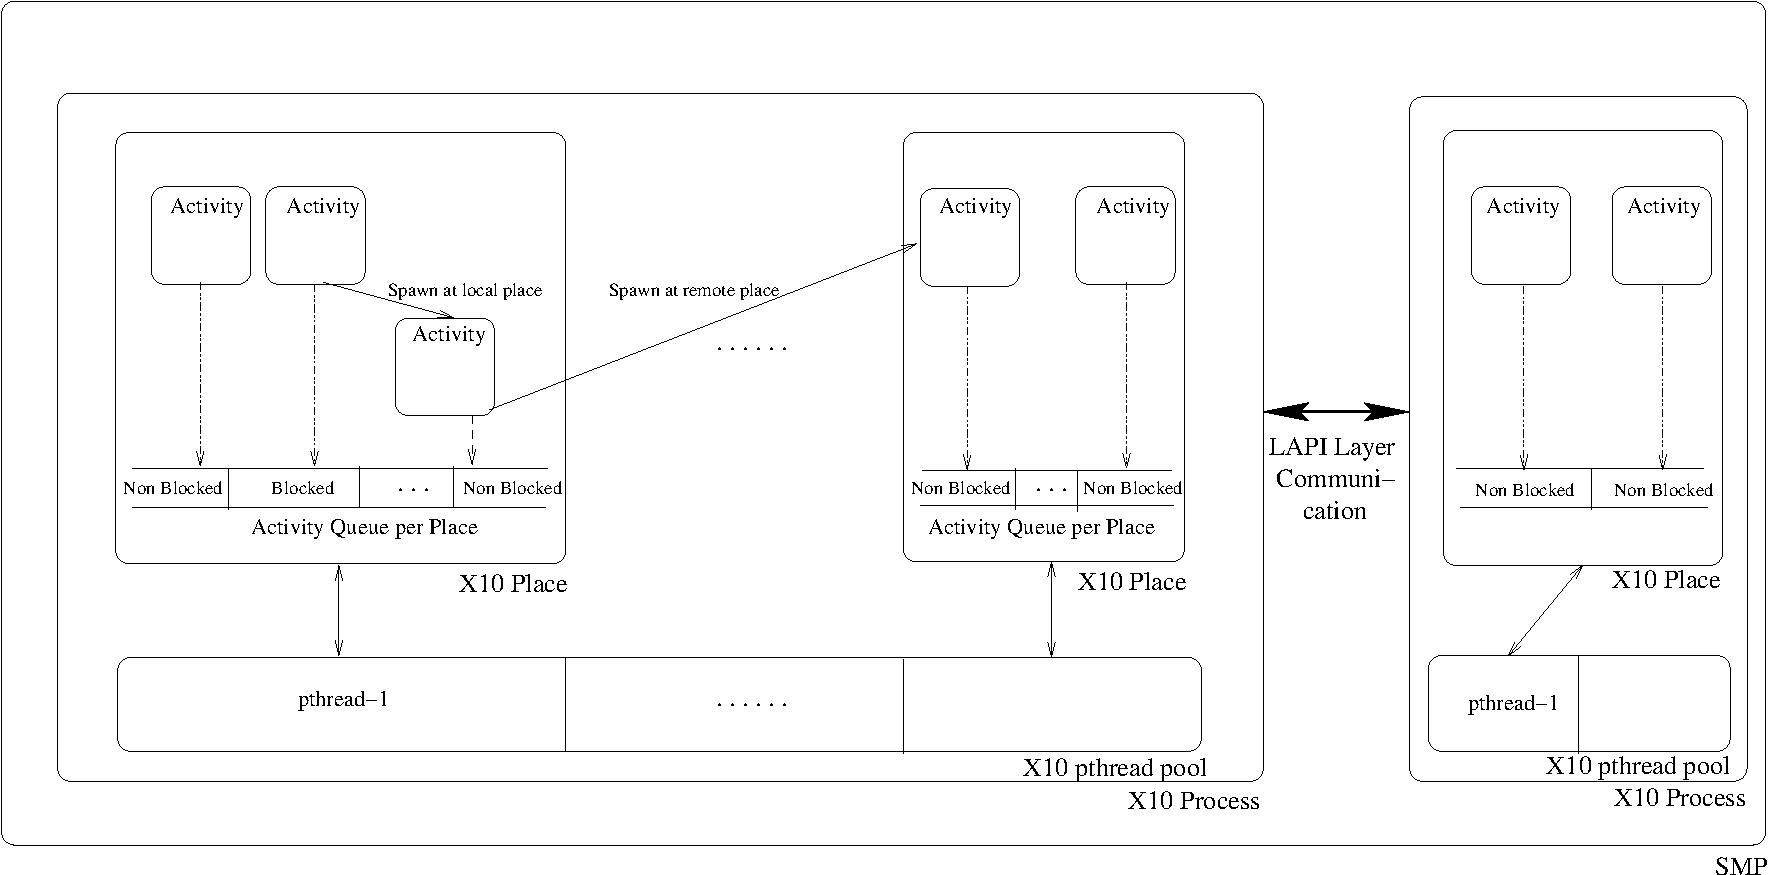
\includegraphics[width=\linewidth]{figs/deploy.pdf}
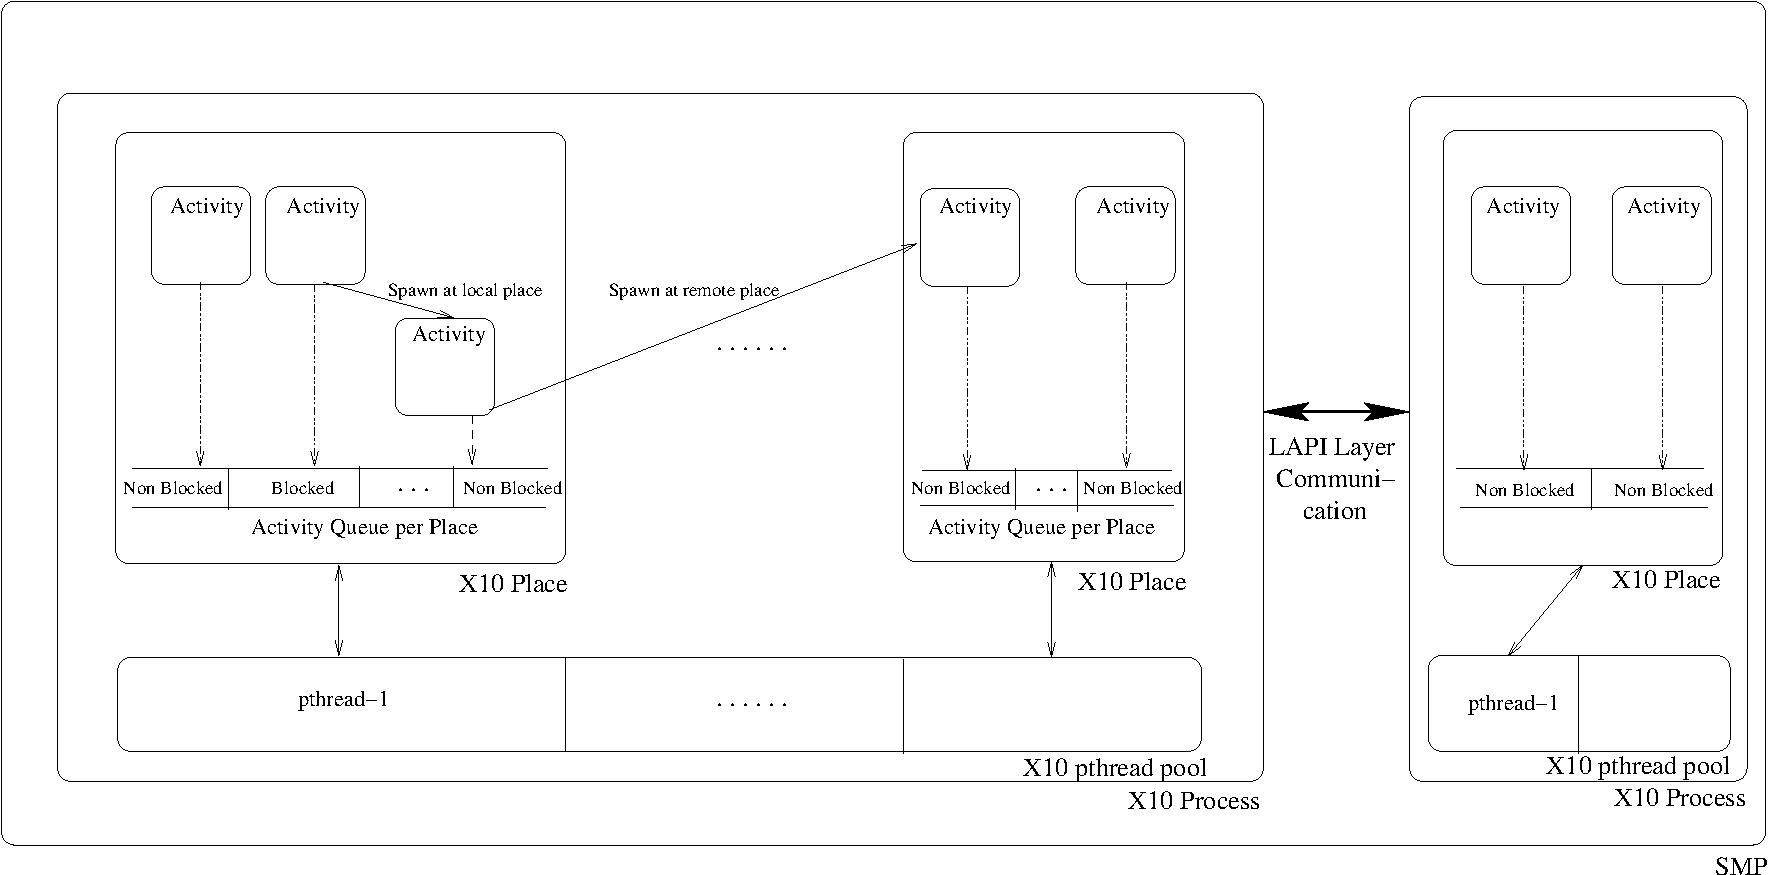
\includegraphics[scale=0.5]{figs/deploy.pdf}
\caption{\Xten{} Deployment on an SMP node}
\label{fig:deploy1}
\end{figure}

\subsubsection{Activities}
\Xten{} programming model allows activities to be either place local or
remote.  These activities can execute any arbitrary code within its body
including blocking operations. The blocking property of an activity is
derived from the fact that it uses one of the following \Xten{}
constructs in : {\it finish}, {\it future-force}, {\it clock-next}, and
{\it atomic-blocks}. In the first iteration, we will allow top-level
blocking activities  and non-blocking activities. Note that top-level
blocking activities are those which does not have a predicated wait in
method body. This information can be determined statically.

Local non-blocking activities may execute like an ordinary function
call.  The compiler may inline such activities.  Local blocking
activities are enqueued in the local activity queue for execution.
During the course of execution if the activity blocks, it suspends its
execution and waits on a predicate of a data structure to be set. As
soon as the predicate of the data structure is set, the blocked activity
is again enqueued and allowed to continue its execution. Remote blocking
activities are enqueued at the destination place's activity queue and
follow the same semantics of blocking as local blocking activities.
Remote non-blocking activities are enqueued at the destination place's
activity queue.


{\bf Operations on Activities:}


\begin{itemize}
\item {\bf Spawning new activities:} New non-blocking child activities
are always allowed to be created. Similarly blocking child
activities are allowed only if they do not have conditional wait in
method bodies. Note that arbitrary blocking activities are not
considered in the first iteration.
\item {\bf Executing blocking operation:} Mark the activity as
blocked in the activity queue  and allow other activities to progress.
\item {\bf Re-enabling blocked activities:} When the predicate of the
data structure is set, the blocked activity is re-enabled in the
activity queue and allowed to proceed with the execution.
\item {\bf Registration on clocks:} Activities during creation or
execution can register with clocks. Clocks keep track
of all activities that are registered on them at a given point of
execution.
\item {\bf Deregistration on clocks:} During execution, activities can
deregister themselves from certain clocks by explicit API calls. This will
implicitly mean that these activities will not participate in
subsequent clock quiescence. 
\item {\bf Resume on clocks:} When an activity invokes {\it resume}
operation on a clock, it intends to say that it has finished
computation of the current phase and moves to the next phase. 
\item {\bf Waiting for clock quiescence:} Activity invoking {\it
next} operation needs to wait for  global quiescence of all clocks
that it is registered with.
\item {\bf Critical region code execution:} Codes protected under
atomic sections are executed exclusively with respect to other
activities within the context of a \Xten{} place. 
\item {\bf Propagate exceptions:} During execution an activity can
throw exception which will be propagated to the innermost {\it finish}
scope.
\item {\bf Collective operations:} A set of activities can participate
in performing an operation collectively i.e., finding the sum of a
distributed \Xten{} array.
\end{itemize}


{\bf Example:}\label{sec:deploy:example}


Consider the following code fragment from RandomAccess benchmark
of HPC Challenge benchmark suite:
\begin{verbatim}
1: finish ateach (point p[i]: ranStarts.distribution) {
2:    long ran = nextRandom(ranStarts[i]);
3:    for (point count: [1:N_UPDATES_PER_PLACE]) {
4:       final int j = f(ran);
5:       final long OK = smallTable[g(ran)];
6:       async(table.distribution[j]) 
7:           atomic {
8:              table[j] = table[j] ^ OK;
9:           } 
10:      ran = nextRandom(ran);
11:   }
12:}	 
\end{verbatim}

The above piece of code updates the {\it table} elements based on a 
randomly computed index. There are two distributed \Xten{} arrays:
{\it ranStarts} and {\it table}. Elements of these arrays are
distributed in the partitioned global address space and is shared
across  SMP nodes, \Xten{} processes, \Xten{} places and \Xten{} 
activities.  Statement~1 creates a number of 
asynchronous activities at various places based on the distribution of 
{\it ranStarts} points. Each of these activities subsequently update
the {\it table} elements in Statements~6-9. The number of updates at 
each place is bounded by a constant {\it N\_UPDATES\_PER\_PLACE} in
Statement~3. Note that {\it smallTable} is not distributed and all 
of its elements are resident in a fixed predefined initial place.
Since the updates to table elements are performed across various \Xten{}
places, Statement~8 is protected in {\it atomic} sections in
Statement~7.

